\begin{frame}[c]
\frametitle{A Theory of Onset Temperature in 2D: Finite-Size Effects at $T \ll T_\mathrm{o}$
} %$J_\sigma$

\begin{columns}[T]

\begin{column}[T]{0.5\linewidth}

\begin{figure}
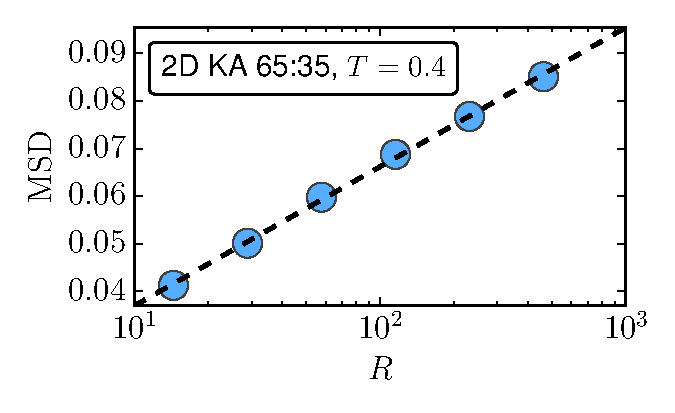
\includegraphics[height=0.5\textheight]{c.10-kt_merminwagner_1/merminwagner_comparison_0.pdf}
\caption{MSD at $t=100 \ll \tau_\mathrm{eq}$. (Shiba, Kawasaki, Kim, \textit{PRL}, 2019).  \onslide<3->{$\km{\sigma_\mathrm{MSD} (k,T)= f(T) \frac{k^2}{2} \approx \textbf{0.25}}$}.}
\vspace{-20pt}
\begin{gather*}
    \mathrm{MSD} \sim f(T) \ln R
    \\
    f(T) = k_{\mathrm{B}} T \frac{\left(3-\nu^{\mathrm{R}}\right)\left(1+\nu^{\mathrm{R}}\right)}{2 \pi Y^{\mathrm{R}}}
\end{gather*}
    
\end{figure}
\end{column}

\begin{column}[T]{0.5\linewidth}

\begin{figure}
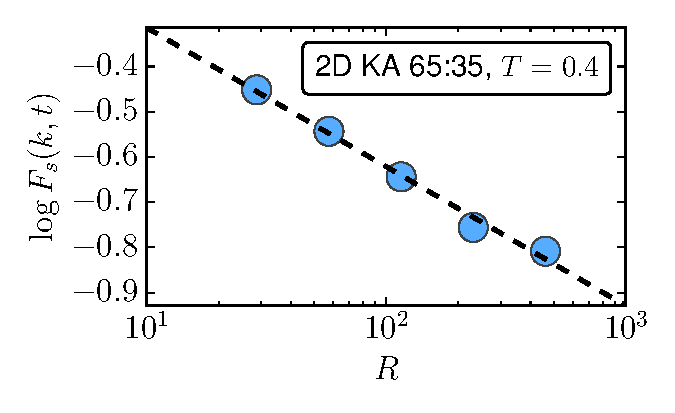
\includegraphics[height=0.5\textheight]{c.10-kt_merminwagner_1/merminwagner_comparison_1.pdf}
\caption{$F_s(k,t)$ at $t=100 \ll \tau_\mathrm{eq}$ and $k\approx 2\pi$. (Shiba, Kawasaki, Kim, \textit{PRL}, 2019). \onslide<2->{$\km{\sigma(k,T) \approx \textbf{0.26}}$}}
\vspace{-20pt}
    \begin{gather*}
    F_{s}\left(k,t \right)  \sim R^{-\frac{\sigma(k, T)}{2}} \\
    \km{\sigma(k, T)} = k_{\mathrm{B}} T \frac{k^{2}\left(3-\nu^{\mathrm{R}}\right)\left(1+\nu^{\mathrm{R}}\right)}{4 \pi Y^{\mathrm{R}}}
    \end{gather*}
\end{figure}

\end{column}

\end{columns}

\end{frame}

% \begin{frame}[c]
% \frametitle{A Theory of Onset Temperature in 2D: Finite-Size Effects MSD} %$J_\sigma$

% \begin{columns}

% \begin{column}{0.45\linewidth}

% \begin{figure}

% \begin{overprint}
% \onslide<4>\centering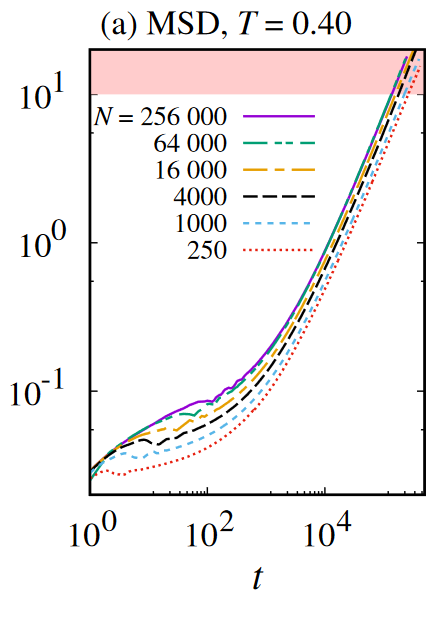
\includegraphics[height=0.75\textheight]{8.d-kt_merminwagner/shiba_msd.png}
% \caption{MSD data from MD simulations (Shiba, Kawasaki, Kim, \textit{Phys. Rev. Lett.}, 2019)}

% \onslide<5-6>\centering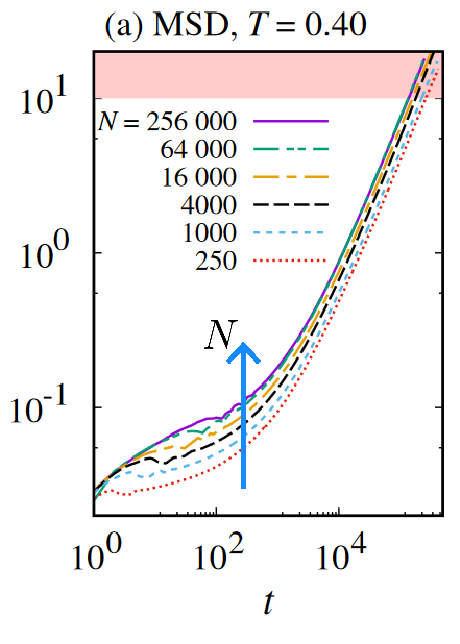
\includegraphics[height=0.75\textheight]{8.d-kt_merminwagner/shiba_msd_witharrow.pdf}
% \caption{MSD data from MD simulations (Shiba, Kawasaki, Kim, \textit{Phys. Rev. Lett.}, 2019)}

% \onslide<7-9>\centering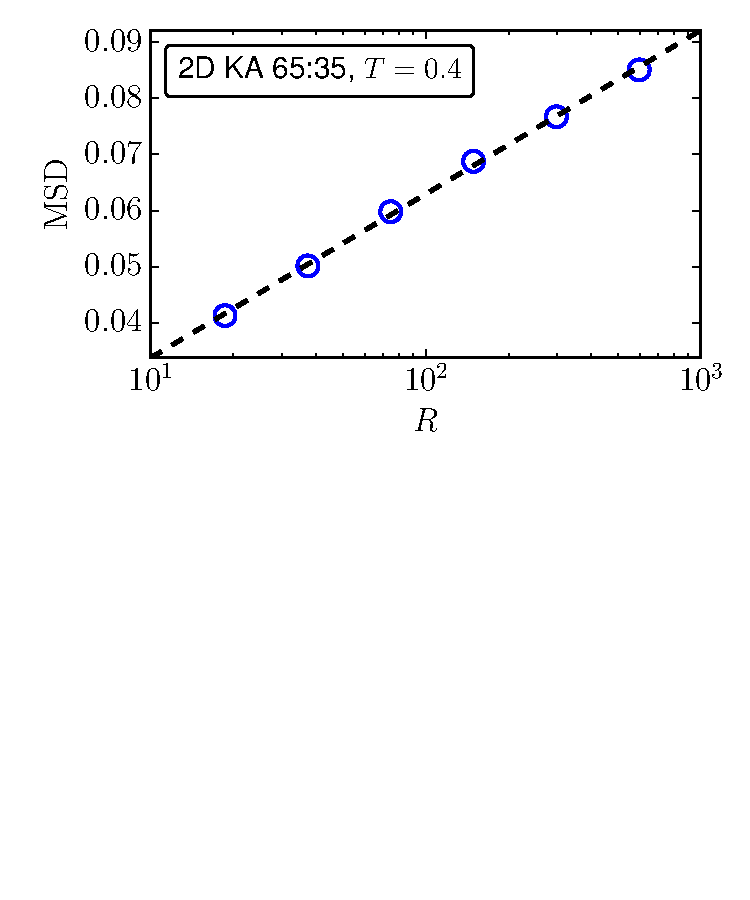
\includegraphics[height=0.725\textheight]{8.d-kt_merminwagner/msd_merminwagner_0.pdf}
% \caption{Replotting MSD at $t=100$ reveals logarithmic finite-size scaling (Shiba, Kawasaki, Kim, \textit{Phys. Rev. Lett.}, 2019)}

% \onslide<10->\centering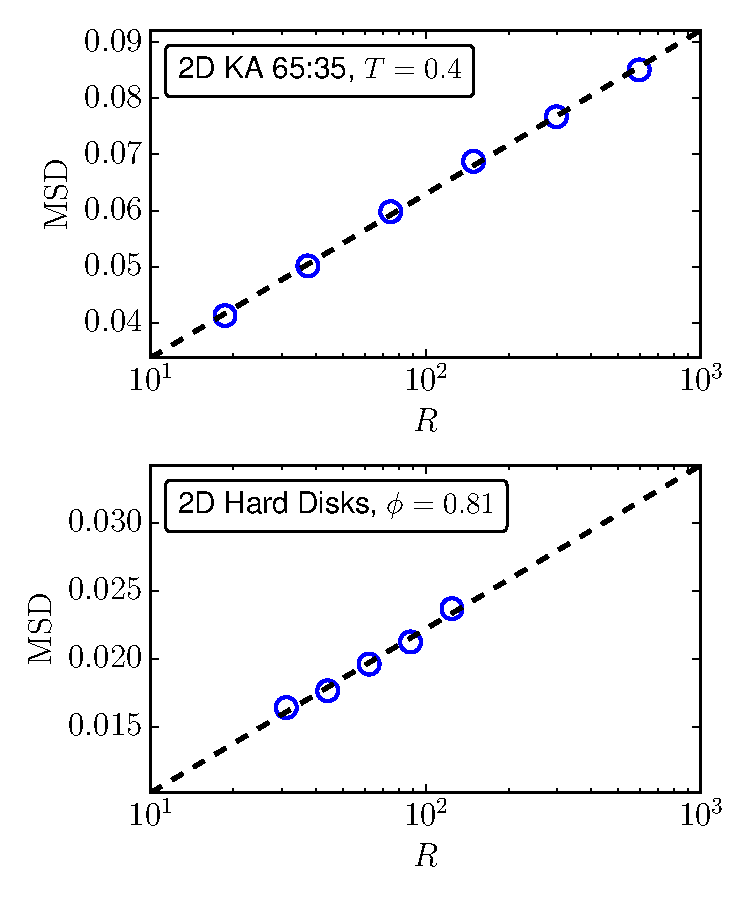
\includegraphics[height=0.725\textheight]{8.d-kt_merminwagner/msd_merminwagner_1.pdf}
% \caption{Logarithmic scaling can also be found in other 2D systems (Illing, et al. \textit{Proc. Natl. Acad. Sci. U.S.A.}, 2017)}
% %\onslide<7->\includegraphics[height=0.4\textheight]{example-image-a}
% %}


% \end{overprint}

% \end{figure}

% \end{column}

% \begin{column}{0.55\linewidth}

% \begin{itemize}
%     \item<2-> Supercooled liquids behave as a 2D solid at intermediate timescales ($t \sim \mathcal{O}(\tau_\mathrm{jump})$) 
%     \item<3-> Displacement fluctuations at $t \sim \mathcal{O}(\tau_\mathrm{jump})$ $\leftrightarrow$ elastic fluctuations (\textbf{Mermin-Wagner}) 
%     \item<6->Our theory yields logarithmic scaling:
%     \onslide<6->
%     {\begin{center}
%     \begin{minipage}{0.85\textwidth}
%     \begin{block}{\centering Finite-Size Effects (MSD)}
%     \begin{gather*}
%     \mathrm{MSD} = f(T) \ln \frac{R}{\xi^{*}} \sim \ln R
%     \\
%     f(T) = k_{\mathrm{B}} T \frac{\left(3-\nu^{\mathrm{R}}\right)\left(1+\nu^{\mathrm{R}}\right)}{2 \pi Y^{\mathrm{R}}}
%     \end{gather*}
%     \end{block}
%     \end{minipage}
%     \end{center}
%     }
%     \item<8-> Depends on \textit{renormalized} elastic moduli! 
%     \item<9->$\xi^*(T)$ is a short-distance cut-off identified from the RG analysis ($\xi^*(T) \to O(\sigma_\mathrm{d})$ as $T \to 0$).
% \end{itemize}

% \end{column}

% \end{columns}

% \end{frame}

% \begin{frame}[c]
% \frametitle{A Theory of Onset Temperature in 2D: Finite-Size Effects $F_s(k,t)$} %$J_\sigma$

% \begin{columns}[T]

% \begin{column}[T]{0.45\linewidth}

% \begin{figure}[t]

% \begin{overprint}
% \onslide<3>\centering\vspace{20pt}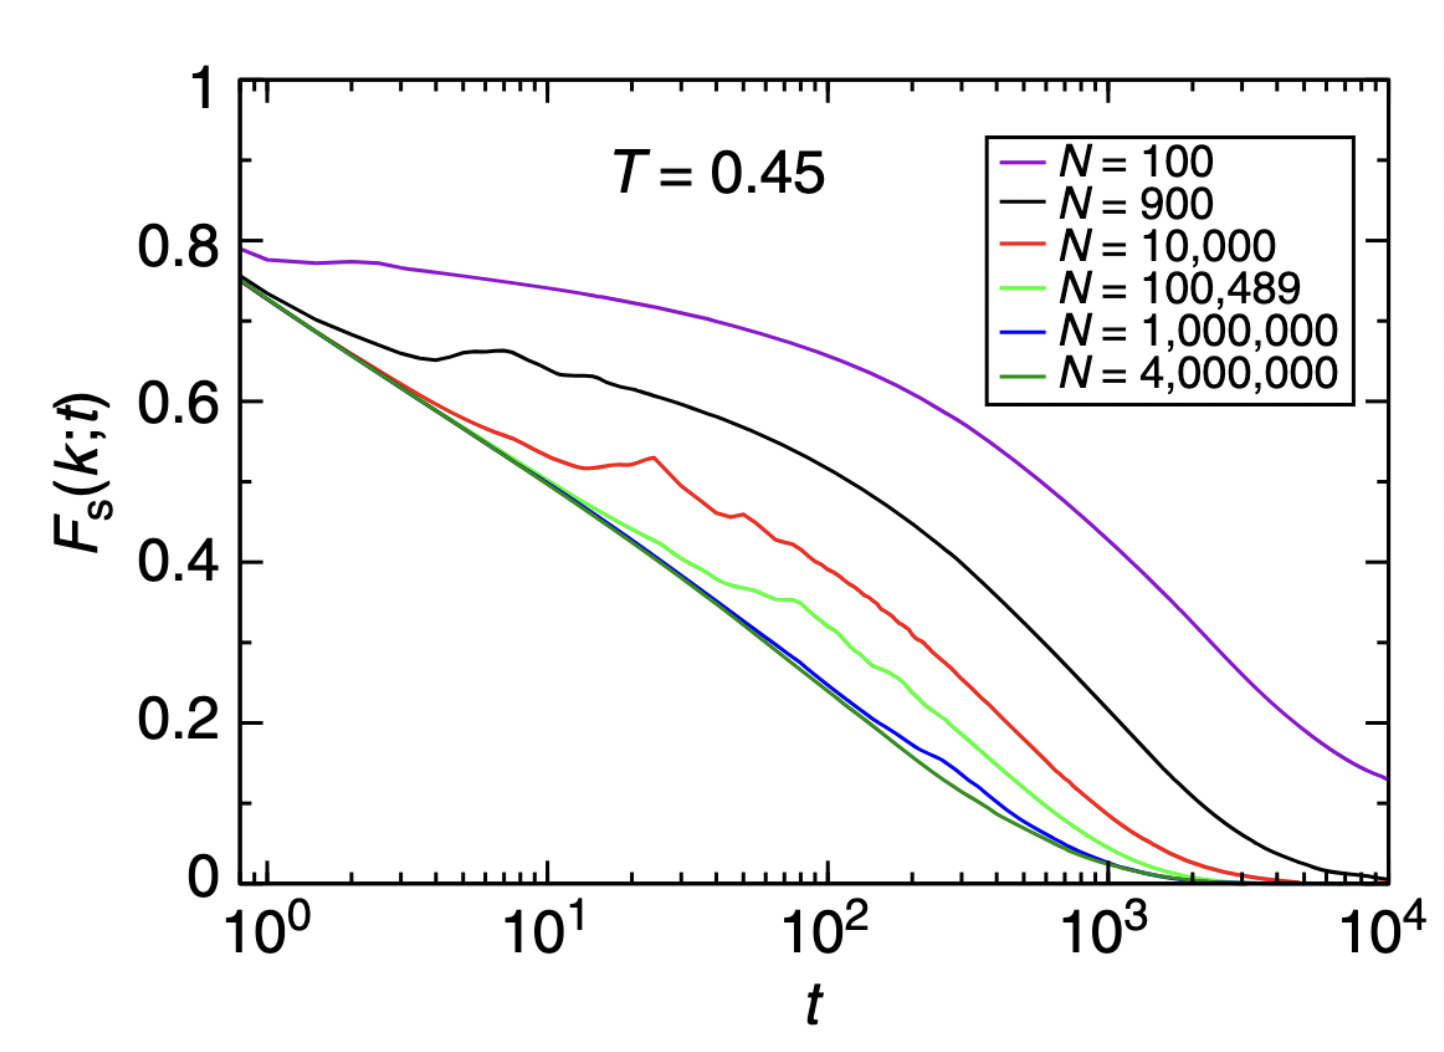
\includegraphics[width=0.9\linewidth]{8.d-kt_merminwagner/fskt_szamelflenner.png}
% \caption{Relaxation proceeds faster as system size is increased (Flenner and Szamel, \textit{Nat. Comm.}, 2015). 2D KA 68:32 system, $k=2 \pi/\sigma_{A}$}

% \onslide<4>\centering\vspace{20pt}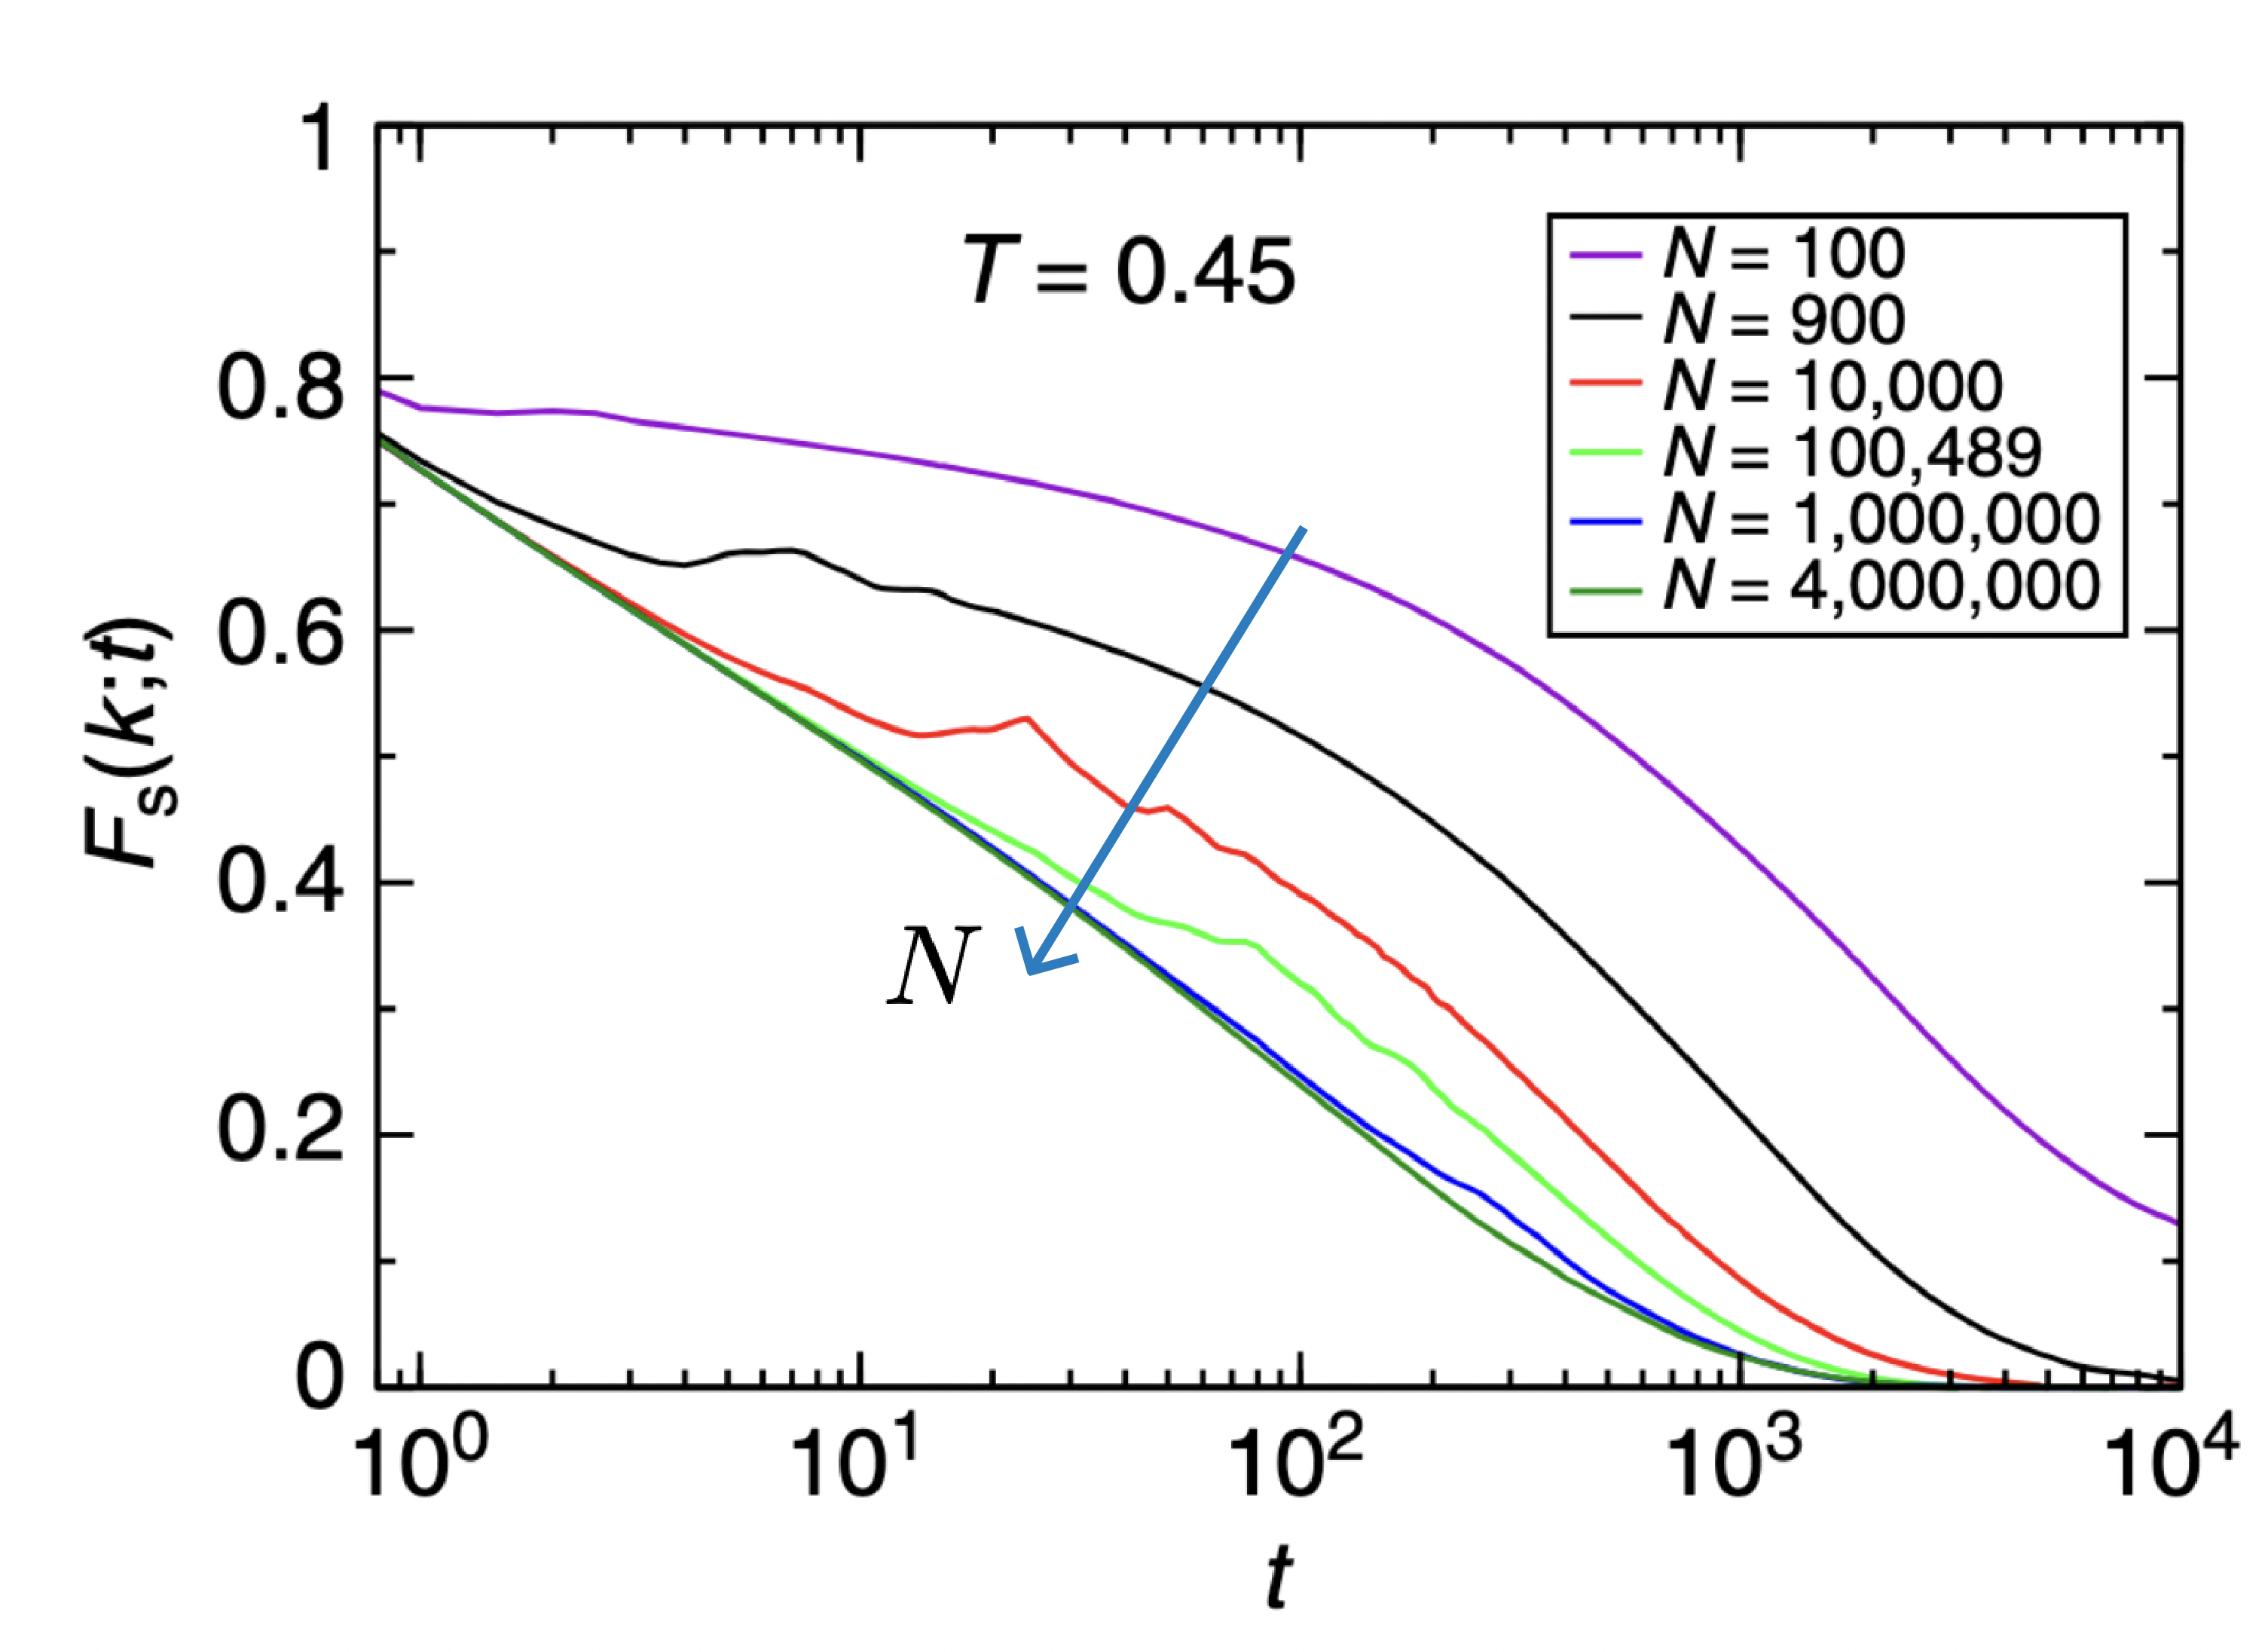
\includegraphics[width=0.9\linewidth]{8.d-kt_merminwagner/fskt_szamelflenner_1.png}
% \caption{Relaxation proceeds faster as system size is increased (Flenner and Szamel, \textit{Nat. Comm.}, 2015). 2D KA 68:32 system, $k=2 \pi/\sigma_{A}$}

% \onslide<5>\centering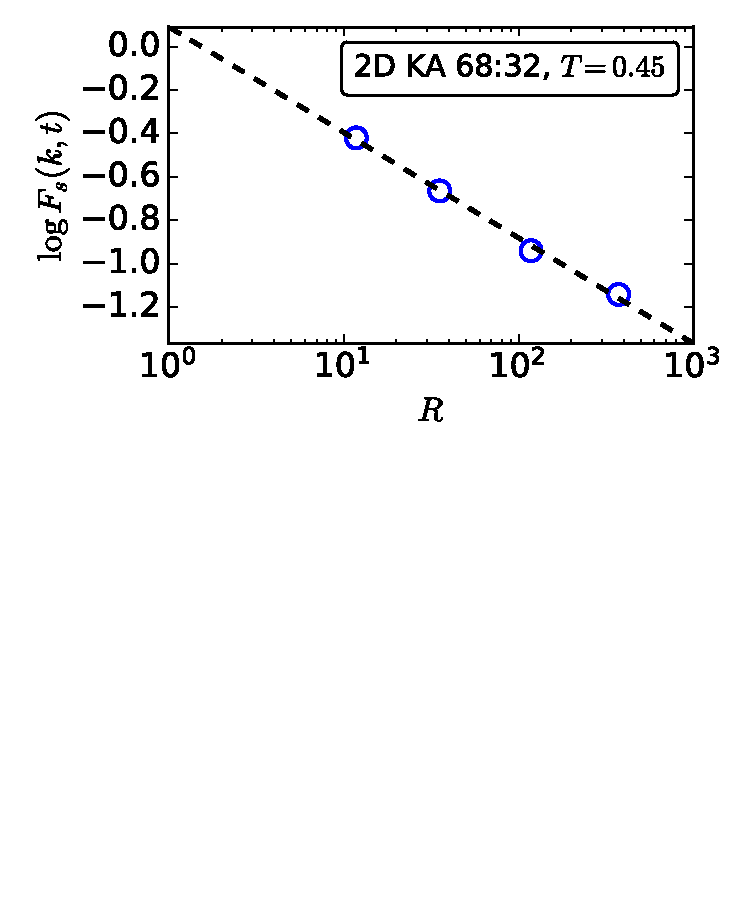
\includegraphics[height=0.725\textheight]{8.d-kt_merminwagner/fskt_merminwagner_0.pdf}
% \caption{Replotting $F_s(k,t=100)$ reveals power-law finite-size scaling (Flenner and Szamel, \textit{Nat. Comm.}, 2015)}

% \onslide<6-7>\centering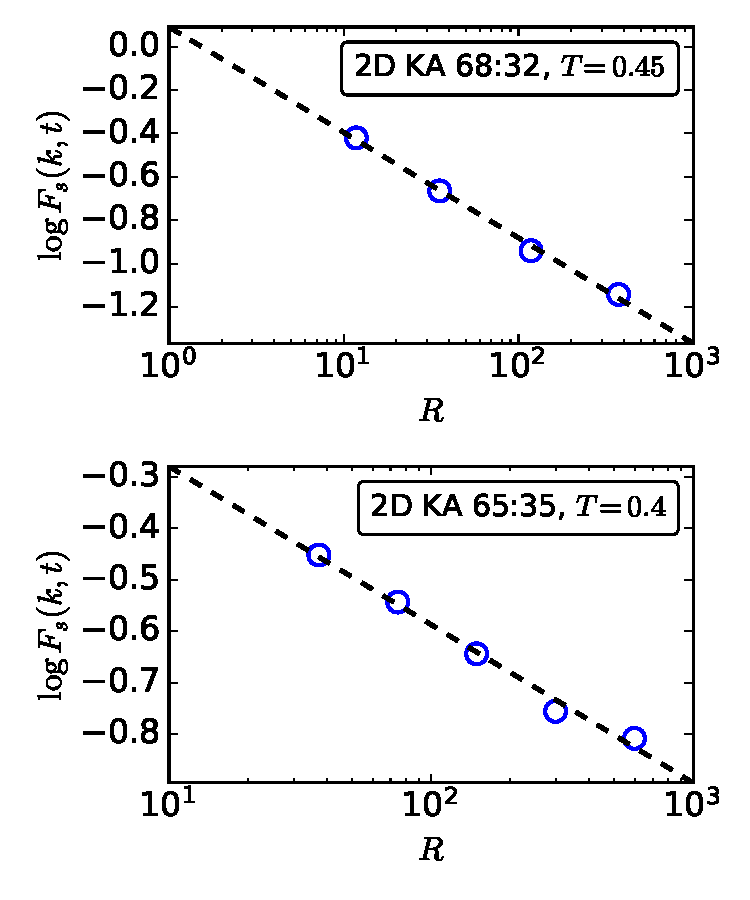
\includegraphics[height=0.725\textheight]{8.d-kt_merminwagner/fskt_merminwagner_1.pdf}
% \caption{Other studies have demonstrated this too (Shiba, Kawasaki, Kim, \textit{Phys. Rev. Lett.}, 2019)}

% \onslide<8->\centering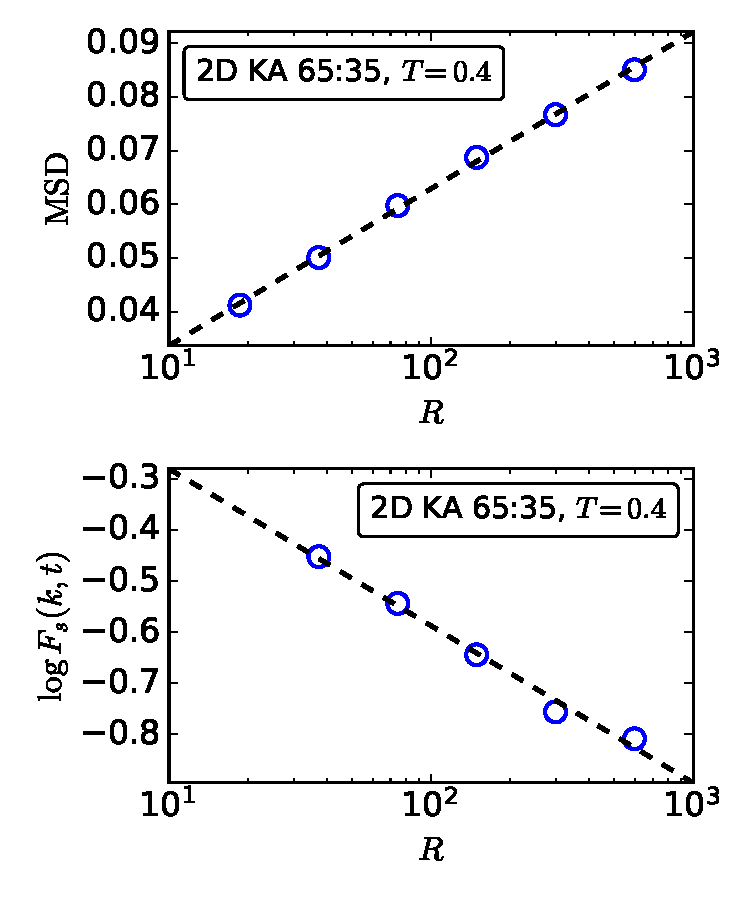
\includegraphics[height=0.725\textheight]{8.d-kt_merminwagner/merminwagner_comparison.pdf}
% \caption{We can estimate the scaling exponent $\sigma(k,T)$ for $F_s(k,t)$ from the MSD}
% %\onslide<7->\includegraphics[height=0.4\textheight]{example-image-a}
% %}


% \end{overprint}

% \end{figure}

% \end{column}

% \begin{column}[T]{0.55\linewidth}

% \begin{itemize}
%     \item<1-> Mermin-Wagner fluctuations impact other measures for relaxation, i.e., intermediate scattering function (density fluctuations).
%     \onslide<2->{
%     \begin{center}
%     \begin{minipage}{0.85\textwidth}
%     \begin{block}{\centering Finite-Size Effects ($F_s(k,t)$)}
%     \vspace{-1em}
%     \begin{gather*}
%     F_{s}\left(k,\left\langle\tau_{\mathrm{jump}}\right\rangle\right)  \simeq\left(\frac{R}{\xi^{*}}\right)^{-\frac{\sigma(k, T)}{2}} \\
%     \sigma(k, T) = k_{\mathrm{B}} T \frac{k^{2}\left(3-\nu^{\mathrm{R}}\right)\left(1+\nu^{\mathrm{R}}\right)}{4 \pi Y^{\mathrm{R}}}
%     \end{gather*}
%     \end{block}
%     \end{minipage}
%     \end{center}
%     }
%     \item<7-> Exponent $\sigma(k,T)$ is related to the prefactor $f(T)$ in the MSD:
%     \begin{equation*}
%     \sigma (k,T) = f(T) \frac{k^2}{2}    
%     \end{equation*}
%     \item<9-> From $F_s(k,t)$: $\sigma(k,T) \approx \textbf{0.26}$. 
    
%     \onslide<10->{From MSD: $\sigma(k,T) \approx (1.26 \cdot 10^{-2}) \frac{k^2}{2} \approx  \textbf{0.25}$.} 
% \end{itemize}

% \end{column}

% \end{columns}

% \end{frame}